\documentclass[12pt,a4paper]{report}

\usepackage[italian]{babel}
\usepackage[utf8]{inputenc}
\usepackage[T1]{fontenc}
\usepackage{listings}
\usepackage[parfill]{parskip}
\usepackage{booktabs}
\usepackage{textcomp}
\usepackage{graphics}
\usepackage{float}
\usepackage{color}
\usepackage{amsmath}
\usepackage{amssymb}
\usepackage{amsfonts}
\usepackage{hyperref}
\usepackage{calc}
\usepackage{enumitem}
\usepackage{subcaption}
\usepackage{footnote}
\usepackage[bottom]{footmisc}
\usepackage{multirow}
\usepackage{threeparttable}
\usepackage{algorithm}
\usepackage[noend]{algpseudocode}
\usepackage{array}
\usepackage{rotating}
\usepackage{setspace}
\usepackage{wrapfig}
\graphicspath{{./images/}}

\usepackage{biblatex}
\addbibresource{bibliography.bib}
\usepackage{csquotes}

%Numbered environment
\newcounter{example}[section]
\newenvironment{example}[1][]{
    \refstepcounter{example}\par\medskip
    \noindent \textbf{Example~\theexample. #1}\newline\rmfamily}
    {\medskip}

\begin{document}

\begin{titlepage}
\begin{onehalfspace}
	\begin{wrapfigure}[4]{l}[22mm]{0.25\textwidth}
		\vspace*{-7mm}
		\centering
		
\includegraphics[width=0.25\textwidth]{bicocca_logo.png}
	\end{wrapfigure}
	\par
	\noindent Università degli Studi di Milano Bicocca \\
	\textbf{Scuola di Scienze \\
			Dipartimento di Informatica, Sistemistica e Comunicazione \\
			Corso di laurea in Informatica}
\end{onehalfspace}

\vfill
\par

\begin{doublespace}
\begin{center}
	{\Huge \textbf{Costruzione Efficiente di Grafi di Splicing}}
\end{center}
\end{doublespace}

\vfill
\par

\begin{onehalfspace}
\begin{flushleft}
	{
	    \large \textbf{Relatore:} \textit{Della Vedova Gianluca} \\
	}
\end{flushleft}

\vspace{8mm}
\par

\begin{flushright}
	{\large \textbf{Relazione della prova finale di:} \\
			\textit{Federico Bergamini} \\
			\textit{Matricola 845646}}
\end{flushright}
\end{onehalfspace}

\vfill
\par

\begin{center}
	{\large \textbf{Anno Accademico 2020 - 2021}}
\end{center}

\end{titlepage}

\thispagestyle{empty}



\cleardoublepage
\begingroup
\let\clearpage\endgroup
\null\vspace{\stretch{1}}

\begin{flushright}
\begin{minipage}{5.3in}
\begin{flushright}
\begin{em}
\section*{Ringraziamenti}
\addcontentsline{toc}{section}{Ringraziamenti}

Al Prof. Della Vedova e alla professoressa Rizzi,
per la fiducia riposta, la pazienza e l'aiuto fornitomi prima, dopo e durante l'esperienza di stage.
\\
Alla mia famiglia,
per avermi supportato (e sopportato) moralmente, psicologicamente ed economicamente in questi tre anni.
\\ 
A tutti gli amici e colleghi, con i quali ho codiviso il mio percorso all'università, per averlo reso unico e speciale.
\\
A chiunque mi abbia consigliato, chiesto aiuto e -soprattutto- criticato, troppi per essere qui elencati, per avermi ricordato che è fondamentale non smettere mai di imparare e migliorarsi.

\end{em}
\end{flushright}
\end{minipage}
\end{flushright}
\vspace{\stretch{2}} \null



\begin{abstract}
    Le nuove tecnologie di sequenziamento producono dati che hanno caratteristiche diverse da quelle che hanno dominato gli ultimi 10-15 anni. 
    In particolare ad oggi vengono prodotte read molto più lunghe (da 10 a 500 volte più lunghe) ma con un tasso di errore più elevato. Ciò richiede di rivedere gli approcci sviluppati in precedenza. 
    Questo stage affronta un importante problema in pangenomica computazionale: ottenere un grafo di variazioni a partire da un allineamento multiplo di long read. 
    Più precisamente, lo stage studierà il problema nel caso ristretto di grafo ottenuto a partire da un insieme di trascritti (grafo di splicing).
\end{abstract}



\tableofcontents

\chapter{Introduzione}
Questa tesi si prefigge l'obiettivo di illustrare ed argomentare l'esperienza di stage maturata durante il terzo anno di laurea triennale nella sua completezza. Verrà posta particolare enfasi sulle motivazioni che mi hanno portato a scegliere questo stage, le tecnologie utilizzate, i concetti teorici alla base, i problemi affrontati con le relative soluzioni e le nozioni da me apprese, oltre che un'introduzione ai concetti di biologia necessari al fine di comprendere al meglio questo elaborato.

\section{Perchè uno stage in Bioinformatica}
Al terzo anno della laurea in Scienze Informatiche dell'università di Milano Bicocca, è chiesto agli studenti di affrontare uno stage su argomenti da loro scelti, al fine di approfondire le conoscenze in materia e acquisire competenze professionalizzanti.


Avendo frequenato l'insegnamento facoltativo di Bioinformatica durante il primo semestre del terzo anno ho avuto la possibilità di appassionarmi alla materia. Nonostante all'inizio la trovassi astrusa, si è rivelata affascinante e mi ha fornito la conoscenza necessaria per portare a temine al meglio l'esperienza di tirocinio.


Ciò mi ha portato a scegliere uno stage difficoltoso, ma stimolante e molto formativo, che affronta un importante problema della pangenomica computazionale : 

La costruzione, in linguaggio Rust, di uno splicing graph a partire da un allineamento multiplo di trascritti in input.

\chapter{Biologia Computazionale}
\label{chap:comp_bio}
Con il termine \textit{Biologia Computazionale} si intende la scienza che si prefigge l'obiettivo di sviluppare ed applicare algoritmi, modelli e metodi matematici al fine di studiare sistemi biologici \cite{Searls19983}. E' una scienza interdisciplinare che attinge a conoscenze di altri campi come matematica, biologia, statistica, biochimica al fine di perseguire i propri obiettivi \cite{AbouttheCCMB}.

Lo sviluppo della biologia computazionale iniziò negli anni 70 del secolo scorso, da allora una sempre più grande mole di dati ed una modesta quantità di pubblicazioni in questo campo, hanno contribuito a rendere questa scienza quella che è oggi.

\section{Obiettivi}
Approcci studiati dalla biologia computazionale sono stati utilizzati per portare a termine vari compiti, tra cui il sequenziamento del genoma umano, creare modelli accurati del cervello umano e dei sistemi biologici.

Alcune sfide che si prefigge la biologia computazionale sono \cite{Searls19983}: 

\begin{itemize}
    \item \textsc{Analisi Struttura delle Proteine.} Capire quali sono le proteine presenti in un campione biologico.
    \item \textsc{Ricerca di omologie nelle sequenze genomiche}
    \item \textsc{Allineamento multiplo di sequenze e ricostruzione di filogenesi.} Analizzare la storia evolutiva di più specie.
    \item \textsc{Analisi di Sequenze.} Comparazione di sequenze genomiche di specie similari o distinte al fine di evidenziare omologie e differenze. Ricostruzione di lunghe sequenze genomiche a partire da frammenti. Correzione di errori da parte delle macchine sequenziatrici. 
\end{itemize}

\section{Bioinformatica}
In particolare la \textit{Bioinformatica} si focalizza sullo studio di tecniche ed algoritmi per l'analisi di strighe (sequenze), applicando e studiando metodi tipici delle scienze informatiche, creando quindi interdisciplinarietà tra le due materie.


Alcuni esempi delle tecniche studiate in Bioinformatica sono:

\begin{itemize}
    \item \textsc{Pattern Recognition.} Identificare una sottostringa all'interno di una più estesa.
        \begin{figure}[h]
        \centering
        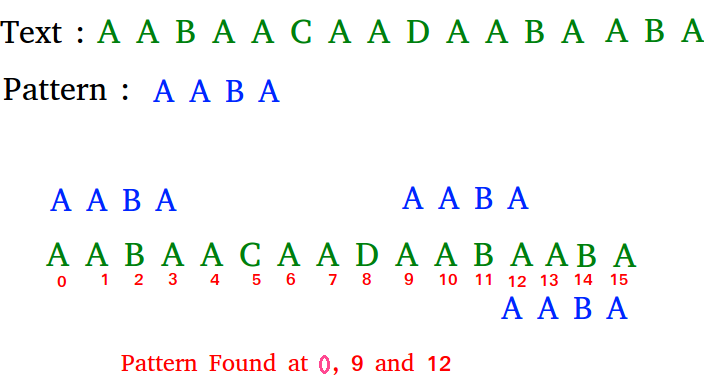
\includegraphics[scale= 0.5]{images/pattern matching.png}
        \caption{Esempio grafico di pattern matching}
        \label{fig:pattern_matching}
        \end{figure}
    \item \textsc{Data Mining}
    \item \textsc{Machine Learning Algorithms}
\end{itemize}

E' da notare che, in realtà, il termine \textit{Bioinformatica} è usato per evidenziare una più ampia gamma di studi inerenti alla biologia che utilizzano approcci informatici per portare a temine i propri obiettivi.

\newpage

\section{Introduzione alla Biologia e Terminologia}
Questa Relazione ha lo scopo di esporre il problema affrontato durante lo stage del terzo anno da un punto di vista informatico. Nonostante ciò verrà fatta un'introduzione ai concetti necessari di biologia molecolare, in modo da facilitare la comprensione di quanto segue.

In biologia Molecolare, la \textit{Trascrizione} è un processo mediante il quale le informazioni contenute nel Dna vengo trascritte su una molecola di Rna.
Un \textit{gene} è una regione del genoma (detta \textit{locus}) che esprime una proteina e viene identificato attraverso il suo \textit{Hugo name} che è un acronimo della sua descrizione.

Si può pensare ad un gene come un'alternanza di regioni codificanti (esoni) e regioni non codificanti (introni).

\begin{figure}[ht]
    \centering
    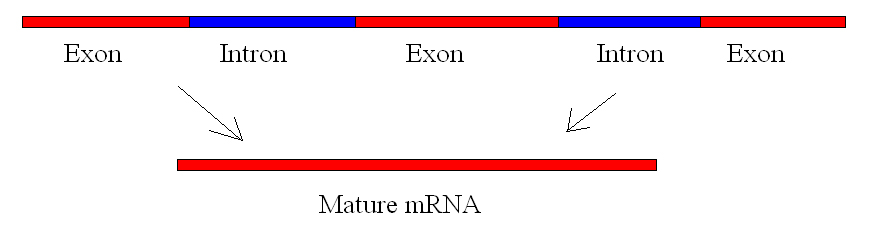
\includegraphics[scale=0.3]{images/introns - exons.jpg}
    \caption{Alternanza di introni ed Esoni}
    \label{fig:intron-exon}
\end{figure}

Il confine tra esone ed introne è detto \textit{Splicing site al 5'}, mentre il confine tra introne ed esone è detto \textit{Splicing site al 3'}.

Quando avviene una \textit{Trascrizione}, il locus del gene viene copiato, compiendo una sostituzione tra le molecole di \textit{Timina} e \textit{Uracile}. Dal punto di vista informatico, il locus è una stringa su alfabeto \textbf{A, C, G, T}, dopo la trascrizione, l'alfabeto diventa \textbf{A, C, G, U} e la molecola formata prende il nome di \newline \textit{pre - mRna}. Successivamente vengono eliminate le regioni non codificanti e viene formata la molecola di \textit{mRna} (trascritto).

%\newpage

I geni umani sono circa 25000, invece le proteine sono centinaia di migliaia. La corrispondenza 1:1 non è rispettata, in quanto un gene può ricombinare i sui esoni in modi diversi al fine di esprimere una molteplicità di trascritti (quindi proteine).
Tutti i trascritti del gene vengono dette \textit{Isoforme di Splicing} del gene.  

\begin{figure}[ht]
    \centering
    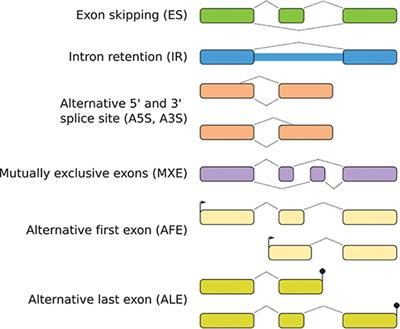
\includegraphics[scale=0.6]{images/alternative splicing.jpg}
    \caption{Esempi di Isoforme di Spliging}
    \label{fig:slicing}
\end{figure}

Studi recenti asseriscono che lo splicing alternativo avvenga sul 90\% dei geni di Homo Sapiens.

Uno dei motivi per cui è utile studiare le isoforme di splicing di un gene, è quello che sono fortemente legate alle malattie.

Patten frequenti dell'alternative splicing sono Exon skiping, Intron Retention, 5' Competing Site, 3' Competing Site, Multiple promoters.



\chapter{Problema della costruzione dello Splicing Graph}
La sfida a cui ho accettato di sottopormi, consiste in un importante problema di pangenomica computazionale, ovvero quello di costruire, in linguaggio Rust, uno splicing graph  a partire da un allineameto multiplo di trascritti di un gene fornito in input. 

Prima di esporre la soluzione al problema, saranno necessari alcuni concetti preliminari, quali quelli di \textit{Allineamento Multiplo} e \textit{Splicing Graph}. Nozioni come \textit{Hugo Name} o \textit{Trascritto} sono già stati forniti nel capitolo \ref{chap:comp_bio}.

\section{Allineamento di Sequenze}
In generale, un allineamento di sequenze è una procedura bioinformatica con cui vengono messe a confronto ed allineate due o più sequenze primarie di aminoacidi, DNA o RNA. L'allineamento permette di individuare regioni identiche o simili che possono avere relazioni funzionali, strutturali o filogenetiche (evolutive). Spesso l'allineamento viene utilizzato per verificare se una sequenza di interesse sia presente all'interno di un database di sequenze conosciute oppure se ne esista una simile. 

Nel caso ristretto dell'allineamento tra due sequenze, quest'ultimo estende il concetto di \textit{Distanza di Hamming} a strighe di lunghezza diversa.

La Distanza di Hamming è definita, solo su strighe di uguale lunghezza, come il numero di posizioni nelle quali i simboli corrispondenti in due stringhe $s_1$ ed $s_2$ divergono. 

In simboli, per distanza, si intende una funzione $d: \mathbb{S}\times \mathbb{S} \to \mathbb{R_+}$, dove $\mathbb{S}$ è l'insieme delle stringhe, che abbia tre proprietà : 

\begin{itemize}
    \item \textsc{Riflessività:} $d(x,y)=0 \iff x=y \textrm{ } \forall \textrm{ } x,y \in \mathbb{S}$
    \item \textsc{Simmetria:} $d(x,y)=d(y,x) \textrm{ } \forall \textrm{ } x,y \in \mathbb{S}$
    \item \textsc{Disuguaglianza Triangolare:} $d(x,y) +d(y,z)\geq d(x,z), \textrm{ } \forall \textrm{ } x,y,z \in \mathbb{S}$
\end{itemize}

Per fare in modo di poter allineare due stringhe con lunghezze diverse, vengono introdotti gli \textit{Indel} (-), che hanno la funzione di "Riempire i buchi". Ci sono due restrizioni nell'iserimento degli indel:

\begin{itemize}
    \item Non possono esistere colonne di soli indel
    \item Le strinche estese di Indel devono avere la stessa lunghezza
    \label{itemize:indel_cond}
\end{itemize}

\begin{example}
$s_1=ABRACADABRA,s_2=BANANA$ \\
Alcuni possibili allineamenti sono:
    \begin{center}
      \begin{tabular}{ c c c c c c c c c c c}
        A & B & R & A & C & A & D & A & B & R & A \\ 
        - & B & - & A & N & A & - & - & - & N & A \\ \hline
        A & B & R & A & C & A & D & A & B & R & A \\ 
        - & - & - & B & - & A & N & A & - & N & A \\ \hline
        A & B & R & A & C & A & D & A & B & R & A \\ 
        - & B & A & N & A & - & - & - & - & N & A \\
      \end{tabular}
    \end{center}
Ciò non significa che siano tutti ugualmente \textit{buoni}
\end{example}

Per saggiare la bontà di un allineamento, è necessario formalizzarlo come un problema di ottimizzazione, quindi definendo:

\begin{itemize}
    \item \textsc{Insieme delle stanze:} Un elemento di $\mathbb{S}\times \mathbb{S}$
    \item \textsc{Insieme delle Soluzioni ammissibili:} gli allineamenti che rispettano le condizioni elencate precedentemente 
    \item \textsc{Funzione Obiettivo:} $\sum_{i=1}^{l} score(s_1[i],s_2[i])$
    \item \textsc{Soluzione:} Allineamento che massimizza l'omologia, quindi la funzione obiettivo
\end{itemize}

Dove $score(s_1[i], s_2[j])$ è il valore del'incolonnamento della colonna presa in esame. Questo valore può essere prelevato da opportune \textit{Matrici di Score} che contengono una funzione $score(c_1, c_2)$ per ogni carattere dell'alfabeto in questione. Ad esempio una matrice di score potrebbe essere \textsc{BLOSUM62} e l'alfabeto $\Sigma=\{A, C, G, T\}$.

\begin{figure}
    \centering
    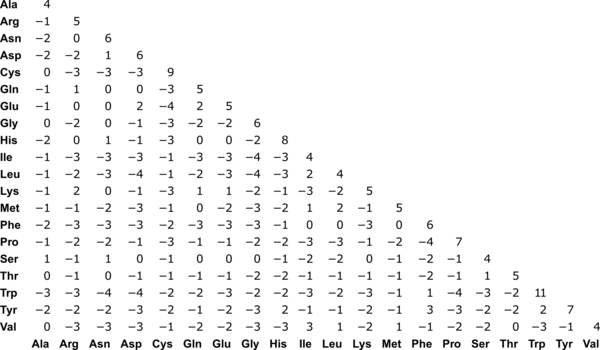
\includegraphics[scale= 0.5]{images/BLOSUM62.png}
    \caption{La matrice di score \textsc{BLOSUM62}}
    \label{fig:blosum32}
\end{figure}

In breve un allineamento può essere interpretato come una misura di omologia tra due o più sequenze. I mismatches possono essere interpretati come punti di mutazione tra le sequenze, invece gli indel o le sequenze di indel (GAP) possono essere interpretate come punti di divergenza nelle sequenze genomiche 

\section{Algoritmi di Allineamento}
Esistono due principali algoritmi che performano allineamenti:  l'algoritmo di Needleman-Wunsch che performa un allineamento globale, cioè allinea le sequenze nella loro interezza e l'algoritmo di Smith-Waterman, che invece performa un allineamento locale, cioè evidenzia regioni simili nelle sequenze genomiche.

\subsection{Algoritmo di Needleman-Wunsch}
L'algoritmo di Needleman-Wunsch utilizza un approccio di programmazione dinamica per risolvere il problema e definisce una equazione di ricorrenza struttutata nel seguente modo : 

\begin{equation*}
    M[i, j] = \textrm{allineamento  ottimo  su }  s1[:i],  s2[:j]
\end{equation*}

\begin{equation}
    M[i, j] = \max  {
                    \begin{cases} 
                        M[i \textrm{-} 1,j \textrm{-} 1] +d(s1[i],s2[j]) & \textrm{nessun indel}\\
                        M[i,j \textrm{-} 1] +d(\textrm{-},s2[j]) & \textrm{indel solo in } s_1\\
                        M[i \textrm{-} 1,j] +d(s1[i],\textrm{-}) & \textrm{indel solo in } s_2\\
                    \end{cases}
                    }
\end{equation}

dove $d(s1[i],s2[j])$ è il punteggio ottenuto dalla matrice di score. Si ricoda che non è contemplato il caso di soli indel in colonna.

Le condizioni al contorno sono:

\begin{itemize}
    \item $M[0,0]=0$
    \item $M[i,0]=M[i \textrm{ - } 1,0] + d(s_1[i],-)$
    \item $M[0,j]=M[0,j \textrm{ - } 1] + d(-,s_2[j])$
\end{itemize}

Il tempo di esecuzione è $\mathcal{O}(nm)$ dove $|s_1|=n$ e $|s_2|=m$.

L'allineamento può essere ottenuto tramite l'usuale \textit{TraceBack} della matrice di programmazione dinamica, partendo da $M[n,m]$ retrocedendo fino a $M[0,0]$.

\begin{figure}[ht]
    \centering
    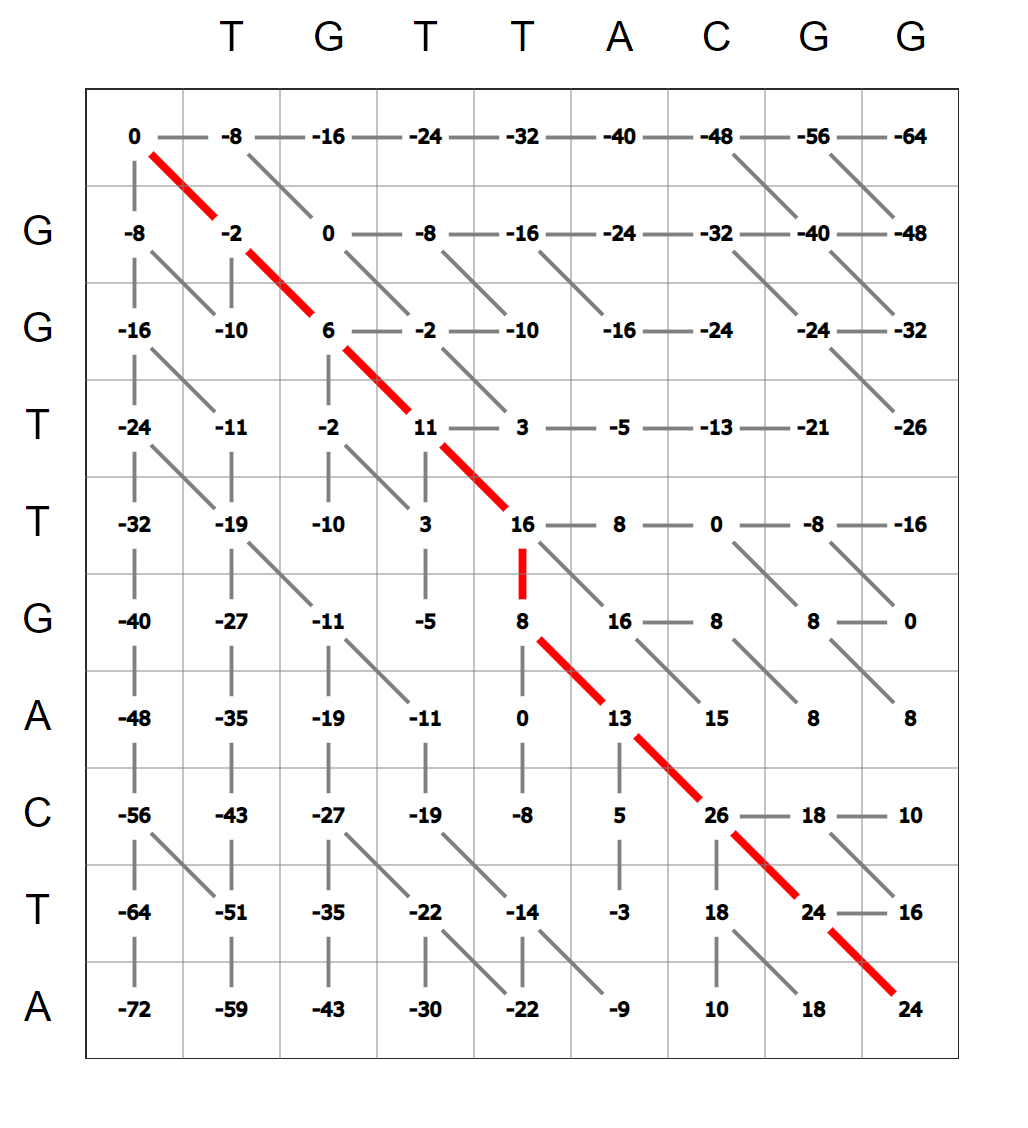
\includegraphics[scale=0.45]{images/esempio nw.PNG}
    \caption{Esempio di esecuzione dell'algoritmo di Needleman-Wunsch su istanza : $s_1=TGTTACGG$ e $s_2=GGTTGACTA$}
    \label{fig:nw}
\end{figure}

\subsection{Algoritmo di Smith-Waterman}
L'algoritmo di Smith-Waterman, come quello di Needleman-Wunsch, utilizza un approccio di programmazione dinamica, ma a differenza di quest'ultimo, evidenzia le sottostringhe di $s_1$ ed $s_2$ che massimizzano il punteggio di allineamento. In altre parole cerca di trovare $t_1=s_1[h:i]$ e $t_2=s_2[k:j]$ tale che il punteggio di allineamento di $t_1$ e $t_2$ sia massimo.

Per raggiungere questo obiettivo pone un limite inferiore al punteggio di allineamento, che non può essere negativo, aggiungendo un nuovo caso all'equazione di ricorrenza dell'algoritmo di Needleman-Wunsch, che si modifica nel seguente modo:

\begin{equation*}
    M[i, j] = \textrm{allineamento  ottimo  su }  s1[:i],  s2[:j]
\end{equation*}

\begin{equation}
    M[i, j] = \max  {
                    \begin{cases} 
                        0\\
                        M[i \textrm{-} 1,j \textrm{-} 1] +d(s1[i],s2[j]) & \textrm{nessun indel}\\
                        M[i,j \textrm{-} 1] +d(\textrm{-},s2[j]) & \textrm{indel solo in } s_1\\
                        M[i \textrm{-} 1,j] +d(s1[i],\textrm{-}) & \textrm{indel solo in } s_2\\
                    \end{cases}
                    }
\end{equation}

dove $d(s1[i],s2[j])$, come in Needleman-Wunsch, è il punteggio ottenuto dalla matrice di score.

Le condizioni al contorno sono differenti da quelle dell'algoritmo di Needleman-Wunsch, in quanto un allineamento non può avere punteggio negativo, e si modificano come segue:

\begin{itemize}
    \item $M[0,0]=0$
    \item $M[i,0]=0 \textrm{ } \forall i \textrm{ } | \textrm{ } 1\leqslant i \leqslant n$
    \item $M[0,j]=0 \textrm{ } \forall j \textrm{ }| \textrm{ } 1\leqslant j \leqslant m$
\end{itemize}

Il tempo di calcolo, come in Needleman-Wunsch, è $\mathcal{O}(nm)$ dove $|s_1|=n$ e $|s_2|=m$.

Il Traceback diventa però più complicato, in quanto deve essere effettuato dal valore massimo della matrice di programmazione dinamica, retrocedendo fino al primo 0.

\begin{figure}[ht]
    \centering
    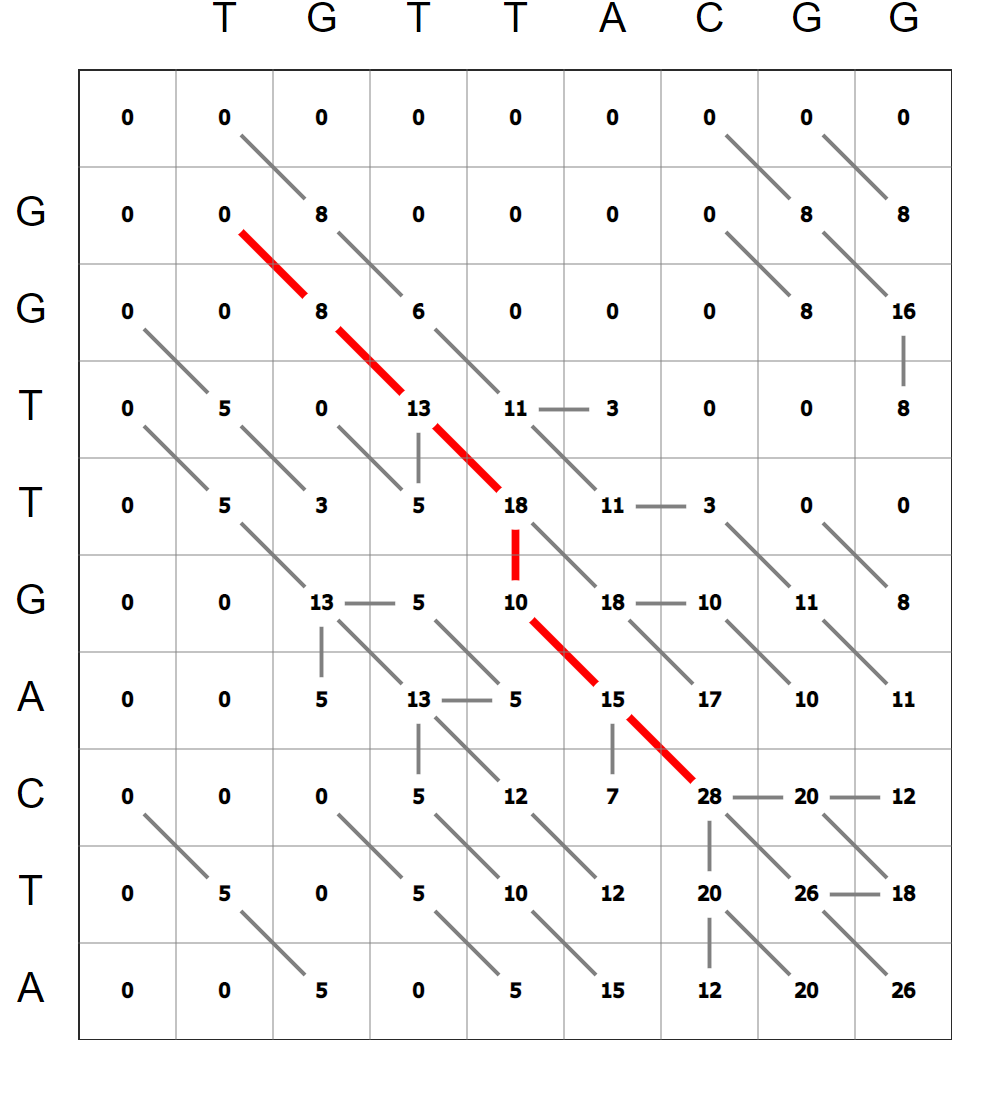
\includegraphics[scale=0.45]{images/esempio sw.PNG}
    \caption{Esempio di esecuzione dell'algoritmo di Smith-Waterman sulla stessa istanza della figura \ref{fig:nw}}
    \label{fig:sw}
\end{figure}

\clearpage
\section{Allineamento multiplo di sequenze}

L'allineamento multiplo è un'esensione del problema dell'allineamento di due sequenze, infatti, l'istanza del problema non sono più due sole strighe, ma un insieme di $k$ stringhe $\mathbb{S}=\{s_1,s_2,s_3,..,s_k\}$.

\begin{figure}[ht]
    \centering
    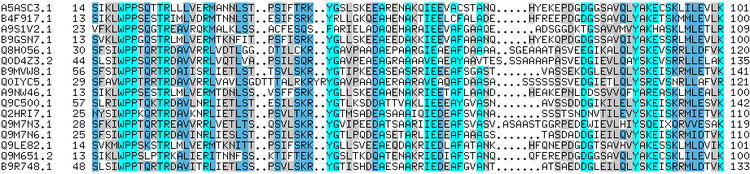
\includegraphics[scale=0.5]{images/multiple sequence alignment.png}
    \caption{Esempio di allineamento multiplo tra sequenze}
    \label{fig:mul_al}
\end{figure}

Ciò però introduce alcuni problemi, ad esempio come posizionare gli indel nelle colonne dell'allineamento. Sicuramente ci potranno essere più indel in una singola colonna, ma non solamente indel, infatti è possibile accettarne fino a $k-1$.

Un altro problema è la funzione codificata nella matrice di score. Infatti essa è una funzione definita $score: \Sigma \times \Sigma \to \mathbb{R_+}$, dove $\Sigma$ è l'alfabeto dei simboli delle stringhe, perciò non può restituire un valore per un numero arbitrario di strighe.

Questo problema è risolto utilizzando la funzione \textit{Sum of Pairs} che somma il punteggio di tutte le righe, prese a coppie, in una colonna di allineamento e ne fa la somma.

Una possibile soluzione al problema dell'allineamento multiplo, è un algoritmo di programmazione dinamica. Questa volta però, a differenza dei due precedenti, l'ultima componente dell'allineamento può trovarsi in $2^k-1$ casi (non è possibile il caso di soli indel).

Il tempo di calcolo è $\mathcal{O}(n^k)$ per un numero contenuto di strighe, altrimenti è \textit{NP-Completo}.

\newpage

\section{Splicing Graph}
Come accennato nel capitolo riguardante la biologia molecolare, lo splicing alternativo è un fenomeno frequentemente osservato che sintetizza vari tracritti dello stesso gene.
Queste varianti possono essere molte e può risultare difficoltoso, specie per i geni più grandi, descrivere le varie isoforme di splicing, con una struttura formale e conveniente che evidenzi le omologie e differenze dei trascritti in input. 

Uno splicing graph cerca di assolvere a questo compito, accorpando, dove possibile, le parti comuni delle sequenze genomiche, dando una descrizione chiara e precisa dei trascritti in input.

\subsection{Definizione Formale ed Esempio}
Uno Splicing Graph è un Grafo Diretto Aciclico (\textbf{DAG}) tale che \cite{bubbles} \cite{spicingest}:

\begin{itemize}
    \item I \textsc{Vertici} rappresentano i siti di splicing per un gene dato. Sono numerati da 1 a n con un identificatore univoco ed etichettati da una sottostringa dei trascritti in input.
    \item Gli \textsc{Archi} rappresentano gli esoni e gli introni tra i siti di splicing. Seguono un ordine crescente degli identificatori univoci dei nodi.
\end{itemize}

Sono aggiunti due nodi "Artificiali" , etichettati con "first\_node" e "last\_node", che hanno come identificatori univoci rispettivamente 1 e n, che segnano i punti di inizio e di fine nella lettura dei trascritti.

\begin{figure}[ht]
    \centering
    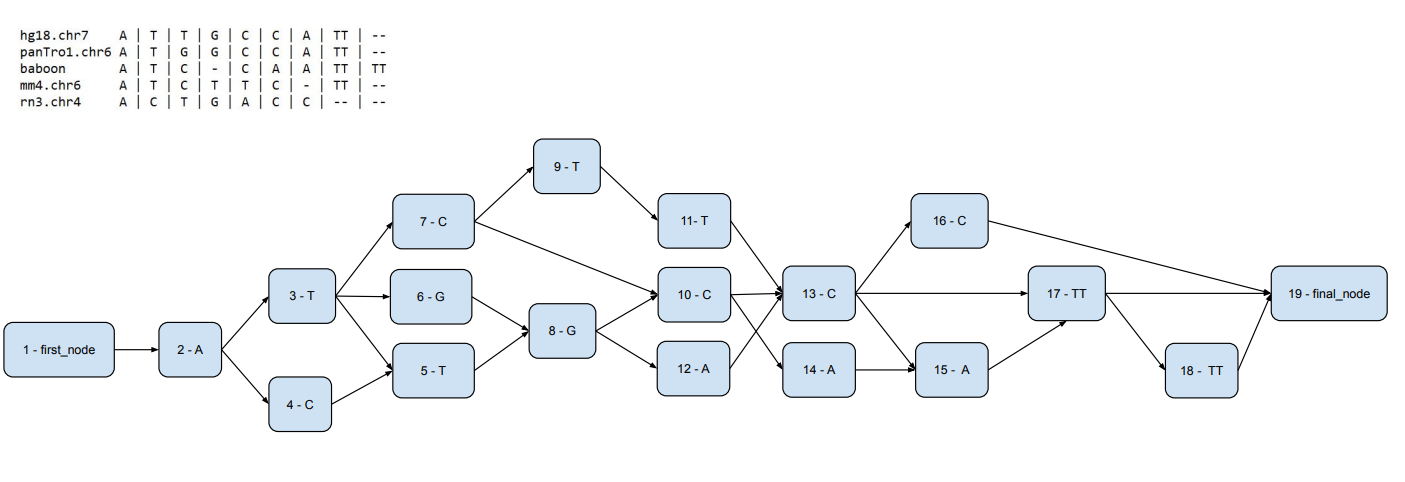
\includegraphics[scale=0.55]{images/Spling graph example.PNG}
    \caption{Esempio di Splicing graph, creato dal mio programma, con l'allineamento multiplo di riferimento}
    \label{fig:slicing_graph_example}
\end{figure}

Non tutti i percorsi $First\_node \to Last\_node$ corrispondo agli effettivi trascritti del gene. Sarebbe necessario limitare il numero di questi falsi trascritti.

\section{Costruzione dello Splicing Graph}
Mi è stato richiesto di implementare una libreria che permetta di creare un grafo di splicing.

In input è fornito un allineamento multiplo di trascritti per fare in modo di evidenziare le omologie tra le isoforme di splicing al fine di rendere più agevole la creazione del grafo. Sono state utilizzate due librerie esterne che permettono di costruire un \textit{Variation Graph} (una generalizzazione dello Splicing Graph) ed eseguire il parsing di file FASTA, uno dei formati standard in bioinformatica, per ottenere l'allineamento multiplo. 

Il parsing di file in formato MAF (Multiple Alignment Format), un altro formato standard in bioinformatica, in assenza di un'alternativa migliore, è stato da me implemementato a partire da una libreria incompleta che lo eseguiva parzialmente.

Nel prossimo capitolo saranno dati i dettagli della soluzione proposta.

\chapter{Soluzione proposta al Problema della costruzione dello Splicing Graph}
Questo capitolo ha lo scopo di illustare la soluzione proposta, i passaggi intermedi ed i ragionamenti logici che mi hanno portato ad elaborare la soluzione finale.

Sarà anzitutto chiarito il perchè del linguaggio \textit{Rust}, definendo le sue particolarità ed i sui punti critici, poi saranno illustrate le pubblicazioni utilizzate per migliorare le soluzioni iniziali, infine verrà eseguita un'analisi dei tempi di calcolo della soluzione definitiva.

\section{Linguaggio Rust}
Il linguaggio Rust è un linguaggio di programmazione sviluppato da Mozilla insieme alla comunità open source per la programmazione di sistemi.

\begin{figure}
    \centering
    
\includegraphics[scale=0.5]{images/rustlang.jpg}
    \caption{Logo del Linguaggio Rust affiancato a quello di Mozilla}
    \label{fig:rustlang1}
\end{figure}

Rust persegue obiettivi di efficienza e sicurezza ed è idoneo allo sviluppo di software concorrente. Sintatticamente simile a \textit{C++}, si differenzia da quest'ultimo a causa del suo meccanismo di salvaguardia della memoria chiamato \textit{Borrow Checker}, che si avvale del design patter \textsc{RAII} (Resource Acquisition Is Initialization) per deallocare le risorse nel caso il loro \textit{Owner} esca di scope \cite{10.5555/3271463}.

Rust non permette l'utilizzo di \textit{null pointer} e \textit{Dangling Reference} che devono essere, in alcuni casi, esplicitamente validati tramite \textit{lifetime}, ciò lo rende un linguaggio sicuro, infatti è stato utilizzato per scrivere alcuni moduli del browser mozilla e parte di alcuni sistemi operativi, tra cui Android.

Rust è usato in bioinformatica, ma in generale in ambito scientifico, perchè oltre alle caratteristiche sopra elencate, è un linguaggio con una buona espressività, simile a quella di un linguaggio a più alto livello, ma più veloce. Ciò lo rende adeguato allo sviluppo di applicativi che necessitano di una buona velocità d'esecuzione e per utenti che non vogliono perdere tempo con gli errori tipici, ad esempio, del C++. Una pecca di rust è che, in generale, è difficoltoso da imparare \cite{whyrust}. 

\section{Soluzione Iniziale}
Prima di poter lavorare sul problema effettivo, c'è stato un preambolo di circa tre settimane in cui è avvenuta una grossa fase di apprendimento. Dapprima ho imparato il linguaggio Rust, poi ho appreso i costrutti resi disponibili dalle varie librerie per adempiere ai miei compiti. In questa fase ho anche creato il parser di file in formato MAF, che è stato un buon esercizio per apprendere ancora meglio Rust.

Terminato questo preambolo, l'approccio che ho deciso di utilizzare per la costruzione dello splicing graph, è stato quello di scansionare l'allineamento colonna per colonna e costruire il grafo di conseguenza. 

In pratica, si assiste ad una fase di inizializzazione, in cui viene creato il nodo 1 con etichetta \textit{first\_node} e aggiunto al \textit{Path} di ogni trascritto nell'allineamento. 

Il costrutto Path è utile in quanto permette di memorizzare i cammini associati ai vari trascritti in termini di sequenza di nodi, quindi di poter associare ad ogni trascritto un percorso attraverso i vertici che corrisponde alla sua sequenza genomica.

In seguito, per ogni colonna dell'allineamento, si costruisce l'insieme dei simboli contenuti, scartando eventuali indel. Per ogni simbolo si costruisce un nodo la cui etichetta è costituita da simbolo stesso e lo si "Aggancia" correttamente al nodo precedente. Dopo aver portato a termine questa operazione, si aggiunge ogni nodo al o ai Path corretti (vedi figura \ref{fig:SplicingGraphConstructionPhases}).

\begin{figure}
    \centering
    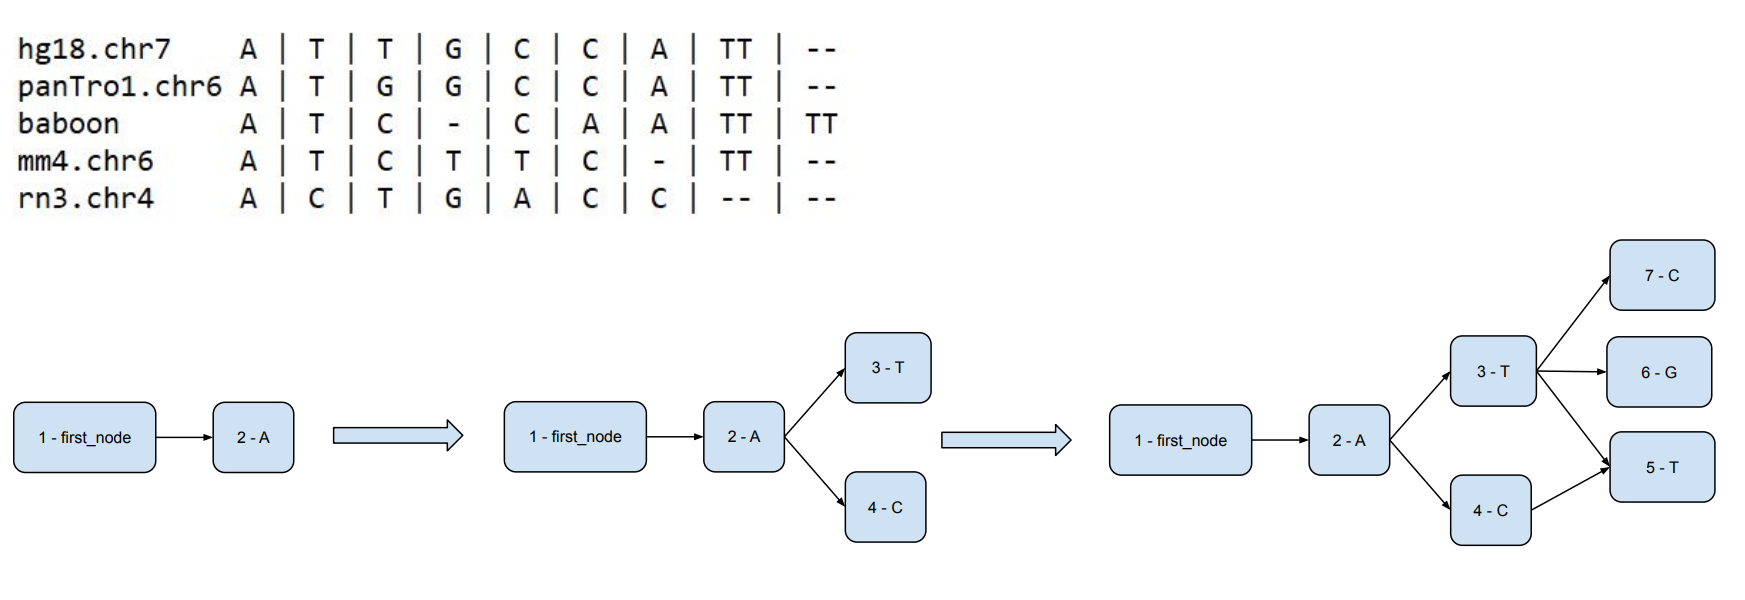
\includegraphics[scale=0.43]{images/Fasi primo approccio.PNG}
    \caption{Le prime tre fasi della costruzione dello Splicing Graph. Vengono prese in considerazione le prime colonne dell'allineamento}
    \label{fig:SplicingGraphConstructionPhases}
\end{figure}

Infine si assiste ad una fase di epilogo in cui tutti i nodi formati nell'ultima iterazione della fase precedente vengono agganciati ad un ultimo nodo etichettato \textit{last\_node}, che corrisponde al nodo di fine e unico nodo foglia del grafo.

Come si può intuire, questo metodo di creazione dello splicing graph, porta alla creazione di un grafo con un eccessivo numero di nodi ed un eccessivo numero di percorsi $first\_node \to last\_node$. Ricordo che, dove possibile, è necessario limitare il numero di questi percorsi.

Una soluzione potrebbe essere quella di seguire lo stesso approccio per la costruzione del grafo, ma invece di considerare l'allineamento colonna per colonna, procedere con un partizionamento opportuno per fare sì di creare dei nodi con etichetta di lunghezza maggiore di 1, in modo da diminuire i nodi già presenti.

La prossima sezione spiegherà le metodologie utilizzate per l'ottenimento di un partizionamento opportuno.

\newpage

\section{Metodologie di partizionamento}
Un buon partizionamento, dovrebbe fare in modo di accorpare il più possibile le colonne dell'allineamento, così da diminuire le quantità di nodi e di percorsi $first\_node \to last\_node$. Per assolvere a questo compito, sono utilizzati due approcci, uno di \textit{programmazione Dimanica} e uno \textit{Greedy}, che originariamente sono stati pensati per risolvere il \textit{Founder Sequence Reconstruction Problem}. Entrambi gli approcci sono descritti in \cite{ukkonen}.

\subsection{Concetti Teorici Preliminari}
Ancora una volta saranno presentati alcuni concetti teorici necessari alla comprensione degli metodi utilizzati per la risoluzione del problema.

Sia $\mathbb{C}=\{C_1,C_2,...,C_m\} \subseteq \Sigma^n$ un insieme di sequenze di lunghezza $n$ su un alfabeto $\Sigma$ detti \textit{Ricombinanti}, ogni ricombinante è scritto come $C_i=c_{i1},c_{i1},...,c_{in}$. Un insieme $\mathbb{F}=\{F_1,F_2,...,F_k\} \subseteq (\Sigma \cup \{\textit{-}\})^n$ è chiamato \textit{Insieme dei Fondatori} per
l'insieme $\mathbb{C}$ e ogni $F_i$ è detta sequenza fondatrice se $\mathbb{C}$ ha un \textit{Parsing} in termini di $\mathbb{F}$. 

Ciò significa che ogni $C_i \in \mathbb{C}$ può essere decomposto in una serie di \textit{Frammenti} non vuoti $f_{ih}$ tale che $C_i=f_{i1}f_{i2}...f_{ip_i}$ e ogni $f_{ih}$ occorre un qualche $F \in \mathbb{F}$ nella stessa posizione in cui è presente anche in $C_i$. 

In altre parole, si può riscrivere $F=\alpha f_{ih} \beta$ dove la lunghezza di $\alpha$ è uguale a quella di $|\alpha|=|f_{i1}...f_{ih-1}|$, mentre la lunghezza di $\beta$ è uguale a quella di $|\beta|=|f_{ih+1}...f_{ip_i}|$.

Si assume che il parsing sia \textit{ridotto} nel senso che due successivi frammenti di $f_{ih}$ e $f_{ih+1}$ siano sempre estratti da elementi diversi di $\mathbb{F}$.

In un parsing (ridotto) di $\mathbb{C}$, si dice che un un ricombinante $C_i$ ha un \textit{Punto di crossover} in $j$ se il parse di $C_i$ è  $C_i=f_i...f_hf_{h+1}...f_{p_i}$ e $|f_1...f_h|=j-1$.

\begin{example}
L'insieme dei ricombinanti:
\begin{center}
  \begin{tabular}{ c c c c c c c c c c c c}
    0 & 0 & 1 & 0 & 0 & 0 & 0 & 1 & 0 & 0 & 1 & 1 \\ 
    1 & 1 & 1 & 1 & 1 & 1 & 1 & 0 & 0 & 1 & 1 & 0 \\
    0 & 0 & 1 & 0 & 1 & 1 & 1 & 1 & 0 & 1 & 1 & 0 \\ 
    1 & 1 & 1 & 1 & 0 & 0 & 1 & 0 & 0 & 0 & 1 & 1 \\
  \end{tabular}
\end{center}

L'insieme dei fondatori:
\begin{center}
  \begin{tabular}{ c c c c c c c c c c c c}
    0 & 0 & 1 & 0 & 1 & 1 & 1 & 0 & 0 & 0 & 1 & 1 \\ 
    1 & 1 & 1 & 1 & 0 & 0 & 0 & 1 & 0 & 1 & 1 & 0 \\
  \end{tabular}
\end{center}
\end{example}

\newpage

A questo punto, il nostro problema è quello di trovare il set di fondatori $\mathbb{F}$ di cardinalità minima, nel contempo massimizzare la lunghezza del frammento più corto $\lambda_{min}$ e la lunghezza media dei frammenti $\lambda_{ave}$. Come è intuitivo pensare, questi sono due obiettivi contradditori.

Ciò ci porta alla formalizzazione di due problemi:

\begin{itemize}
    \item Il primo è il \textsc{minimum founder set problem} che consiste nel trovare il set di fondatori $\mathbb{F}$ di cardinalità minima tale che il parse di $\mathbb{C}$ in termini di $\mathbb{F}$ abbia $\lambda_{min} > L$ oppure $\lambda_{ave} > L$ per un L dato chiamato \textit{Threshold}.
    
    \item Il secondo è il \textsc{maximum fragment length problem} che consiste nel massimizzare $\lambda_{min}$ e/o $\lambda_{ave}$ sotto la condizione che la cardialità di $\mathbb{F} \leq M $ per un M dato.
\end{itemize}

Al fine di costruire uno Splicing Graph, è sembrato più congeniale, modellare il problema a partire dal \textsc{minimum founder set problem}, in quato si è voluta tenere più bassa possibile la cardinalità di $\mathbb{F}$. Ciò ha portato ad un buon grafo, a cui possono essere fatte ulteriori migliorie.

\subsection{Soluzione di Programmazione Dinamica}
Un algoritmo risolutivo del minimum founder set problem è basato sull'idea di segmentare l'insieme dei ricombinanti $\mathbb{C}$ in segmenti disgiunti, in modo da partizionare interamente $\mathbb{C}$. Un segmento $C[j,k]$ è definito come l'insieme di tutte le sottosequenze $c_{ij}...c_{ik}$ dell'insieme dei Ricombinanti. 

Il nostro obiettivo diventa quindi quello di dare un parsing di $\mathbb{C}$ con $\lambda_{min} > L$ per un L dato, tale che la cardinalità massima dei segmenti sia minimizzata, ciò minimimizza anche la cardinalità dell'insieme $\mathbb{F}$ dato che $|\mathbb{F}|=|\max\{C[j,k]\}|$

Si vuole quindi computare:

\begin{equation*}
    M(n)=\min_{s \in S_L}\{|C[j,k]| : |C[j,k]| \in s \} 
\end{equation*}

Dove s è l'insieme dei partizionamenti possibili su $\mathbb{C}$.

Quindi $M(n)$ può essere ottenuto valutando $M(L),M(L+1)...M(n),$ nel seguente modo:

Caso base:

\begin{equation*}
    M(L)= |C[1,L]| 
\end{equation*}

Passo Ricorsivo:

\begin{equation*}
    M(j)= \min_{h \leq j-L} \max_{j=L+1,...,n} \{M(h),|C[h+1,j]|\}
\end{equation*}

Il tempo di calcolo per questo approccio è $\mathcal{O}(n^2m)$ dove $n$ è la lunghezza dell'allineamento e $m$ è il numero delle sequenze allineate.

Con l'usuale traceback dell'array di programmazione dinamica,, è possibile giungere al partizionamento corretto.

Questa soluzione non tiene però conto degli indel presenti nelle sequenze. 

E' opportuno o meno contare sottosequenze che presentano solo indel nella cardinalità dei segmenti? o ancora; è opportuno contare le sottosequenze formate solo parzialmente da indel?

Come conseguenza della soluzione greedy presentata nella prossima sezione, sono arrivato alla conclusione che non ha senso il conteggio di una sottosequeza di soli indel nella cardinalità di un segmento. Invece ha senso il conteggio di una sottosequenza formata solo parzialmente da indel.

In generale questa, soluzione di programmazione dinamica, non restituisce risultati ottimali.

In particolare, con allineamenti di sequenze troppo diverse tra di loro, si assiste ad un partizionamento praticamente inesistente, nel senso che, in un caso limite, si verrà a formare un grafo con $n+2$ vertici, con etichette corrispondenti alle intere sequenze in input, che corrispondono alle $n$ sequenze in aggiunta al nodo etichettato $first\_node$ e a quello etichettato $last\_node$.

La soluzione greedy cerca di ovviare a questo problema.

\newpage

\subsection{Soluzione Greedy}

La soluzione greedy, anch'essa descritta in \cite{ukkonen}, ha come obiettivo quello di trovare il partizionamento con il minor numero di segmenti tale che ogni segmento abbia cardinalità massima $M$.

Tale obiettivo è raggiunto considerando inizialmente $|C[1,k]| \leq M$ poi progressivamente $|C[k+1,k']| \leq M$ fino al termine dell'allineamento, tale che i partizionamenti siano più lunghi possibile.

Questa soluzione è però fin troppo semplicistica, infatti non contempla il fatto che un segmento di cardinalità 1 potrebbe già superare la soglia $M$. 

Che fare in questo caso?

Si potrebbe pensare di scegliere $M$ opportunamente, in modo da non permettere a questo caso di presentarsi. Dovrebbe essere sufficiente inserire un valore di $M \geq \min \{|\Sigma|,n\}$ dove $n$ è il numero delle sequenze e $|\Sigma|$ è la cardinalità dell'alfabeto su cui sono costruite le stringhe.

Questo tipo di soluzione porterebbe però, in alcuni casi, a segmenti troppo lunghi, quindi a non accorpare al meglio l'allineamento.

Al fine di poter mantenere un valore di $M>0$, inizialmente ho pensato di interrompere il segmento nel caso $|C[k,k+1]| > M$. Però ciò portava ad un grafo come quello mostrato in figura \ref{fig:primo_esempio_splicing_graph_greedy}.

\begin{figure}[ht]
    \centering
    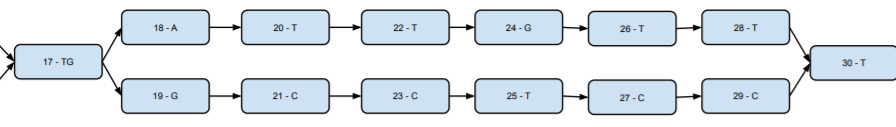
\includegraphics[scale=0.7]{images/greedy1.PNG}
    \caption{Primo Esempio di soluzione greedy. Per comodità, è riportato solo un frammento del grafo}
    \label{fig:primo_esempio_splicing_graph_greedy}
\end{figure}

Logicamente si vorrebbero accorpare i nodi 18, 20, 22, 24, 26, 28 in un unico nodo, così come i vertici 19, 21, 23, 25, 27, 29.

Ciò è possibile se si permette all'algoritmo di partizionamento, in certi casi, di non attenersi al vincolo di cardinalità dei segmenti. I casi in questione sono proprio quelli menzionati in precedenza, infatti se il segmento di cardinalità minima già eccede $M$, allora gli è permesso accorpare più colonne dell'allineamento fino a quando non aumenta ulteriormente di cardinalità, o quando non è possibile formare un nuovo frammento di cardinalità minore. Allora si inizia un nuovo frammento.

Nel conteggio di cardinalità dei segmenti sono omesse le sottosequenze di soli indel, esattamente come nell'algoritmo di programmazione dinamica menzionato nella sezione precedente.

Questo "Nuovo" algoritmo greedy permette di formare un grafo come quello in figura \ref{fig:greedy_definitivo}.

\begin{figure}[ht]
    \centering
    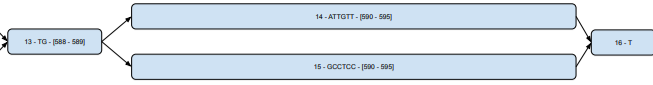
\includegraphics[scale=0.9]{images/greedy2.PNG}
    \caption{Esempio definitivo di soluzione greedy. Per comodità, è riportato solo un frammento del grafo e sono riportati gli indici dell'allineamento corrispondenti alle etichette dei nodi}
    \label{fig:greedy_definitivo}
\end{figure}

\newpage

\section{Soluzione Definitiva}
Tra il primo approccio e l'approccio definitivo si sono susseguiti numerosi tentativi. Ad esempio, nelle prime soluzioni, il calcolo nella cardinalità dei segmenti includeva anche le sequenze di soli indel, in seguito ciò è stato cambiato. 

Per una maggiore chiarezza espositiva non verranno mostrati tutti i tentativi eseguiti, ma solo il primo e l'ultimo.

Avendo un partizionamento adeguato, costruito mediante soluzione greedy o di programmazione dinamica, la corstruzione del grafo risulta molto simile a quella del primo approccio. 

La fase di inizializzazione è identica a quella precedentemente descritta, come la fase di terminazione, mentre quella di costruzione vera e propria deve tenere conto che non si ragiona più in termini di simboli, ma in termini di sottostringhe dell'allineamento. 

Innanzitutto si itera sul partizionamento e per ogni segmento se ne estrae la cardinalità e l'insieme delle sottosequenze contenute, in seguito, per ognuna di queste, si crea un nodo che viene concatenato al precedente nodo correttamente, infine viene aggiunto al path corretto.

Per avere un'idea più chiara della costruzione del grafo, si può comunque fare riferimento alla figura \ref{fig:SplicingGraphConstructionPhases}, in quanto la costruzione avviene incrementalmente come mostrato. Verrà comunque fornita un'immagine contenente il codice Rust della procedura di costruzione del grafo (\ref{fig:build_vg}).

I valori di soglia, $M$ se si preferisce la soluzione greedy, o $L$ se si preferisce quella di programmazione dinamica, sono impostabili dall'utente, ma è consigliato tenerli bassi in entrambi i casi, per fare in modo di costruire un grafo migliore. Ad esempio, nella figura \ref{fig:greedy_definitivo}, è stato scelto il valore $M=1$, quindi l'algoritmo greedy di partizionamento.

\begin{figure}
    \centering
    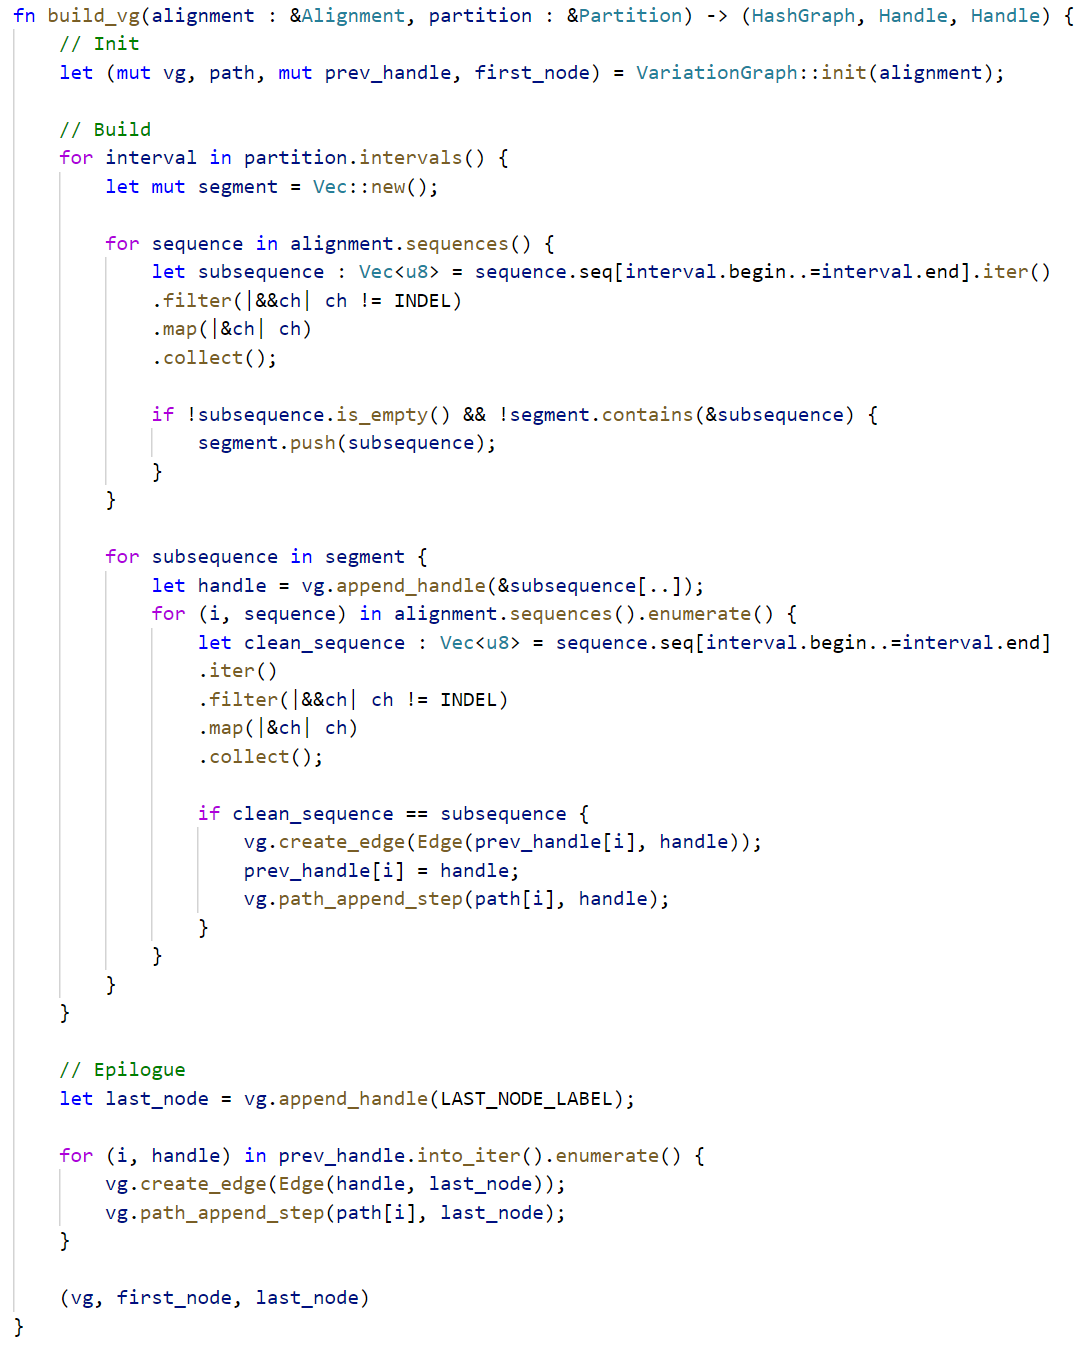
\includegraphics[scale=0.7]{images/build_vg.PNG}
    \caption{Procedura Rust di costruzione del Grafo di Splicing}
    \label{fig:build_vg}
\end{figure}

\newpage

\section{Tempi di Calcolo}
Fare un'analisi formale dei tempi di calcolo risulterebbe difficile, in quanto dipende da diversi fattori quali il tipo di partizionamento utilizzato, la lunghezza dei segmenti formati e il numero di sequenze in input.  

La fase di preprocessamento delle sequenze, in cui viene estratto il partizionamento, ha tempi diversi a seconda del partizionamento utilizzato, in particolare:

\begin{itemize}
    \item \textsc{Greedy} : il tempo di esecuzione è $\mathcal{O}(nm)$.
    \item \textsc{Programmazione Dinamica} : il tempo di esecuzione è $\mathcal{O}(n^2m)$.
\end{itemize}

La vera e propria procedura di costruzione de grafo, è scomposta in tre fasi separate:

\begin{itemize}
    \item \textsc{Fase di inizializzazione} che prende un tempo $\mathcal{O}(n)$ dove $n$ è il numero delle sequenze, in quanto deve inizializzare i path per ogni sequenza e inserire $first\_node$ per ognuno di questi.
    \item \textsc{Fase di costruzione} che, come si può vedere in figura \ref{fig:build_vg} prende un tempo che è proporzionale al numero di segmenti formati durante il pre-processamento, e al numero di sequenze in input. inoltre è proporzionale alla cardinalità del segmento preso in considerazione alla data iterazione del ciclo più esterno.
    In sistesi si potrebbe pensare ad un $\mathcal{O}(k(n + nm))$ dove $n$ è il numero dei trascritti, $k$ è il numero dei segmenti, $m$ è la cardinalità del segmento.
    \item \textsc{Epilogo} che prende un tempo $\mathcal{O}(n)$ dove $n$ è il numero delle sequenze, in quanto deve finalizzare i path per ogni sequenza e inserire $last\_node$ per ognuno di questi.
\end{itemize}

In ogni caso viene complicato stabilire i tempi con accuratezza perchè, ad esempio la lunghezza dei segmenti diminuisce le iterazioni del ciclo più esterno, ma potrebbe allungare i tempi per il confronto delle sottostringhe.

\newpage

\section{Architettura del Software}
Questa sezione è dedicata ad esporre l'architettura definitiva del software prodotto.

Verrà introdotta la struttura software del parser MAF e di quello Fasta, dopo di che verrà introdotta la struct \textit{Partitioner} che si occupa del partizionamento e infine la struct \textit{VariationGraph} che si occupa della costruzione e visualizzazione del grafo.

\subsection{I parser MAF e FASTA}

\begin{figure}[ht]
    \centering
    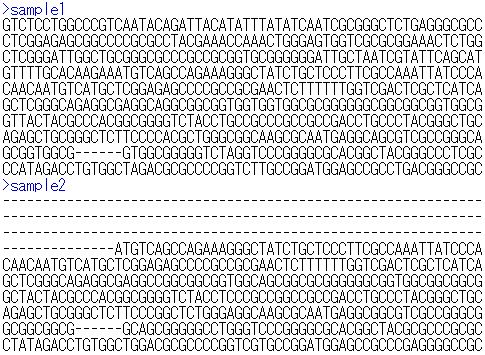
\includegraphics[scale=0.5]{images/fasta example.png}
    \caption{Esempio di allineamento memorizzato su file FASTA}
    \label{fig:fasta_alignment}
\end{figure}

\begin{figure}[ht]
    \centering
    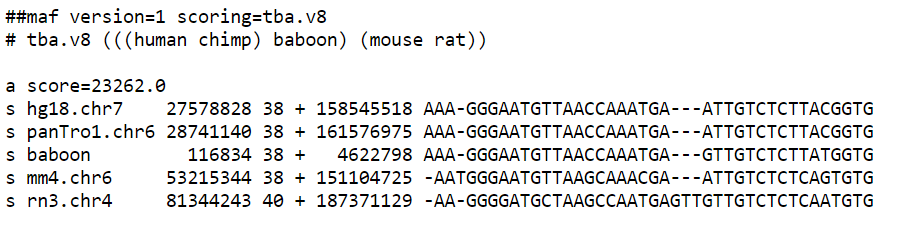
\includegraphics[scale=0.7]{images/Maf file example.PNG}
    \caption{Esempio di allineamento memorizzato su file MAF}
    \label{fig:maf_alignment}
\end{figure}

Il parser Maf si avvale di una serie di struct ed enum, ognuna relativa ad un particolare elemento del file MAF. 

Le prinipali sono:

\begin{itemize}
    \item \textsc{MAFItem}: una enum che rappresenta un elemento del file MAF, quindi un commento od un blocco di allineamento.
    
    \item \textsc{MAFBlock}: una struct che rappresenta un blocco di allineamento che contiene un vettore di \textit{MAFBlockEntry} e una mappa contenente i metadati di intestazione del blocco.
    
    \item \textsc{MAFBlockAlignedEntry} è una struct che rappresenta uno dei due tipi di \textit{MAFBlockEntry}, questa struct contiene effettivamente la sequenza di basi allineate e l'identificativo della sequenza
\end{itemize}

Il paser Fasta si avvale di una libreria chiamata RustBio che performa il parser per noi.

Siccome i due parser producono oggetti differenti, è stato necessario "unificarli" in un unico oggetto che contiene solo le informazioni necessarie ai fini della costruzione dello splicing Graph.

Questo oggetto è stato chiamato \textit{Alignment} e contiene :

\begin{itemize}
    \item Le effettive sequenze allineate 
    \item Per ogni sequenza viene memorizzato anche l'identificativo univoco
    \item Un metodo per stampare su file l'allineamento nel caso sia necessario.
\end{itemize}

Al fine di agevolare il parsing da ulteriori formati di file, nel caso ce ne fossero, è stato inserito un trait denominato \textit{Parser}. Si può vedere un trait come un'interfaccia java che può fungere da linea guida, nel nostro caso, per lo sviluppo di ulteriori parser.

Inoltre è inserita una enum che incapsula gli errori che possono verificarsi al momento del parsing, ad esempio un file non trovato, oppure un file che non contiene nessun allineamento.

\newpage

\subsection{Partitioner}
La struct \textit{Partitioner} si occupa dei eseguire il partizionamento dell'allineamento multiplo. Per assolvere a questo compito si avvale di alcuni costrutti aggiuntivi.

\begin{figure}[ht]
    \centering
    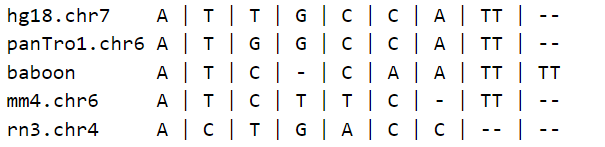
\includegraphics[scale=1]{images/partitioning_example.PNG}
    \caption{Esempio di partizionamento su un'istanza semplice del problema}
    \label{fig:partitioning_example}
\end{figure}

Come descritto nel capitolo precedente, il partizionamento viene eseguito da due algoritmi differenti che utilizzano due strategie diverse, perciò è sembrato opportuno definire un trait chiamato \textit{Partitioner} che fungesse da linea guida per lo sviluppo delle struct effettive che effettuano il partizionamento.

Per la rappresentazione del partizionamento è stata scelta una classe che contiene un vettore di elementi di tipo \textit{Inerval}. Interval è una struct congeniale allo scopo di una rappresentazione più chiara di un singolo segmento, si compone di un indice di inizio, chiamato \textit{begin} e un indice di fine chiamato \textit{end} che rappresentano rispettivamente l'inizio e la fine di ogni segmento.
Gli intervalli sono sempre disgiunti e crescenti.

La struct che performa il partizionamento in prorammazione dinamica è denominata \textit{DynProgPartitioner}. Questa struct si preoccupa di eseguire i controlli sul parametro \textit{threshold} al fine di accertarne la validità, inoltre performa l'effettivo algoritmo di programmazione dinamica.

Per quanto riguarda quest'ultimo, per agevolare il traceback dell'array di programmazione dimanica, viene utilizzata una struct aggiuntiva, chiamata \textit{Cell}, che contiene l'effettivo valore del partizionamento, ma anche un campo previous che è utile nella ricostruzione dei segmenti.

Al momento del traceback, vengono formati gli intervalli del partizionamento.

La struct che invece performa l'algoritmo greedy, è chiamata \textit{GreedyPartitioner}. Questa struct performa il partizionamento nel modo descritto nel capitolo precedente, iterando sull'allineamento e verificando che i segmenti siano di cardinalità minore di \textit{threshold}. Se la cardinalità diventa maggiore, cerca di allungare il segmento il più possibile fino a quando non si accorge che si potrebbe formare un segmento di cardinalità minore o che potrebbe ampliarla uteriormente.

Per il calcolo della cardinalità di ogni segmento, viene utilizzato un metodo comune, dato che viene fatto nello stesso modo.

\newpage

\subsection{VariationGraph}
La struct \textit{Variation Graph} si occupa della costruzione dello splicing graph a partire da un partizionamento in input. Il partizionamento è ottenuto utilizzando il metodio greedy o di programmazione dinamica.

La struct \textit{Variation Graph} contiene i riferimenti a first\_node e last\_node e un \textit{HashGraph} che rappresenta l'effettivo grafo. HashGraph è un tipo di dato importato una una libreria esterna.

Il metodo \textit{build\_vg} si occupa della corstruzione progressiva del grafo a partire dal partizionamento in input, si avvale del metodo init per inizializzare tutti i \textit{Path} relativi alle sequenze e l'array dei predecessori per ogni sequenza input. 

Il metodo build\_vg itera sulle partizione formate in precedenza per fare in modo di creare correttamente il grafo e i path contenenti i nodi correttamente etichettati e connessi. L'array dei predecessori è utile per tenere conto di quale nodo è presente nel path della sequenza associata, in modo da "Agganciare" correttamente il successivo.

La costruzione si conclude con un epilogo in cui ad ogni path è aggiunto il nodo last\_node.

La struct VariationGraph contiene anche altri metodi quali : 

\begin{itemize}
    \item \textsc{print\_path}: che stampa a schermo il path associato all'identificativo della sequenza passato come parametro.
    
    \item \textsc{get\_possible\_path}: che restituisce il numero di percorsi \newline $first\_node \to last\_node$. Questo metodo inizialmente è stato pensato come un metodo ricorsivo che si avvale di una funzione aggiuntiva per calcolare il numero di cammini possibili. Questo approccio però portava ad un tempo di esecuzione proporzionale al numero dei cammini presenti nel grafo, come si può vedere in figura \ref{fig:slow_get_path_num}.
    
    \begin{figure}[ht]
        \centering
        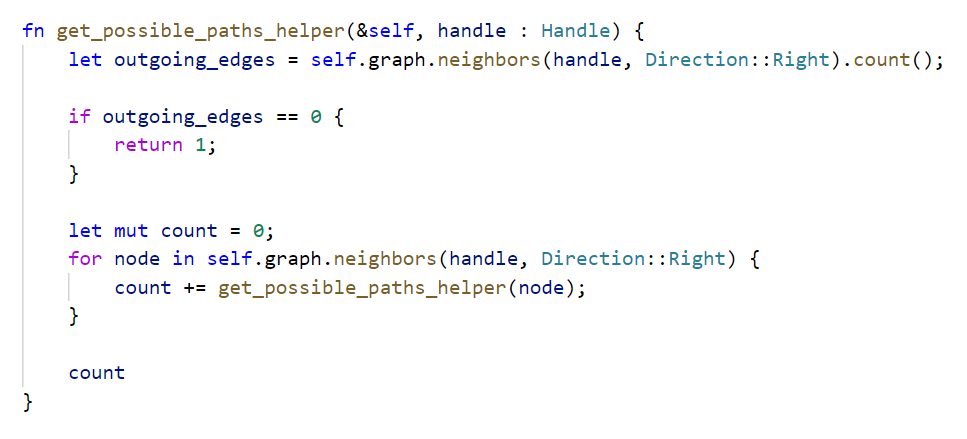
\includegraphics[scale=0.6]{images/slow_path_count.PNG}
        \caption{versione del metodo $\mathcal{O}(|paths|)$}
        \label{fig:slow_get_path_num}
    \end{figure}
   
    Di seguito, come mostrato in figura \ref{fig:fast_get_path_num} è utilizzato un metodo di simil-programmazione-dinamica, che sfrutta il fatto di memorizzare il numero dei cammini che partono da un dato nodo e arrivano a last\_node per rendere il tempo di esecuzione proporzionale al numero dei nodi, che è, in generale, molto inferiore a quello dei cammini.
    
    \begin{figure}[ht]
        \centering
        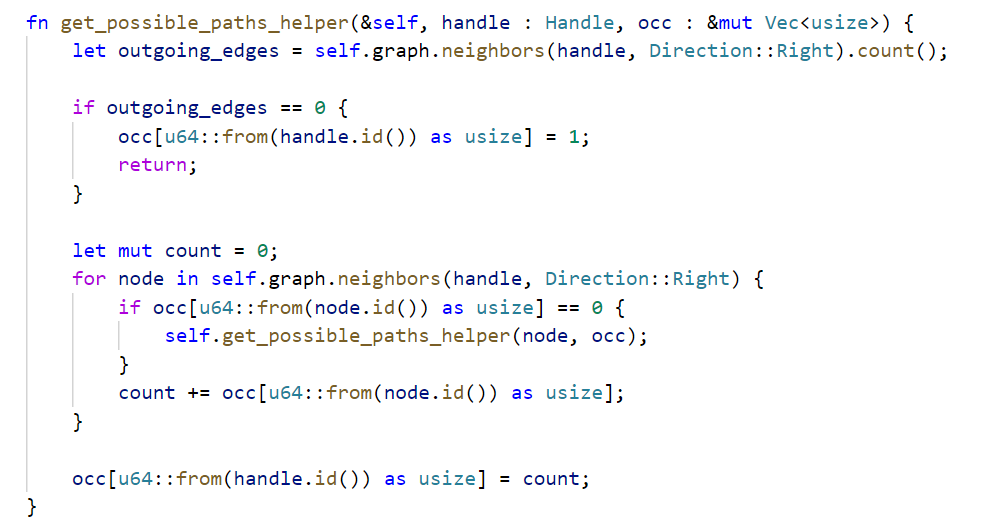
\includegraphics[scale=0.6]{images/fast_path_count.PNG}
        \caption{versione del metodo $\mathcal{O}(|V|)$}
        \label{fig:fast_get_path_num}
    \end{figure}
    
    \item \textsc{label\_len\_sum} : che restituisce la somma delle lunghezze delle etichette dei nodi del grafo.
    
    \item \textsc{print\_graph} : che stampa il grafo in un modo opportuno. In particolare, per ogni nodo nel grafo stampa : 
    
    \begin{itemize}
        \item L'identificativo univoco
        \item L'etichetta associata
        \item I nodi entranti
        \item I nodi uscenti
    \end{itemize}
\end{itemize}

\newpage

Nella figura \ref{fig:construction_example} verrà fatto un esempio di costruzione di splicing graph per dare un'idea migliore di come funziona l'architettura software creata.

\begin{figure}[ht]
    \centering
    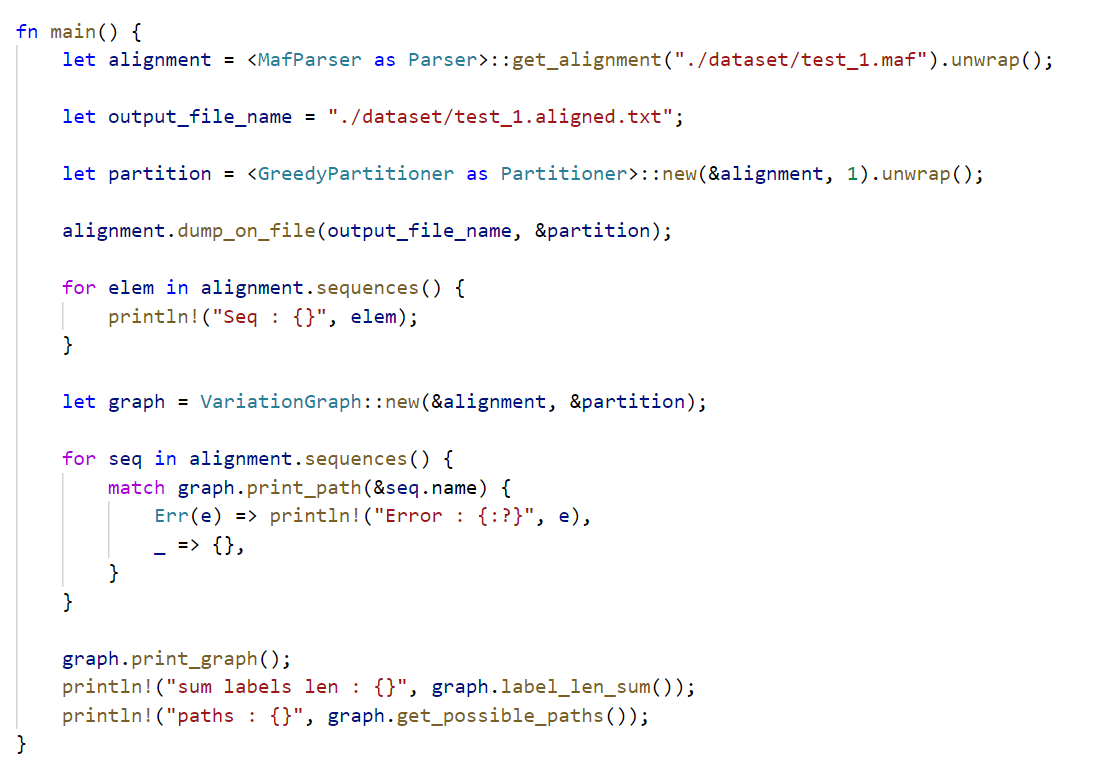
\includegraphics[scale=0.6]{images/main example.PNG}
    \caption{Esempio di costruzione del grafo di splicing}
    \label{fig:construction_example}
\end{figure}

\clearpage

\subsection{Test}
Oltre alle struct sopra descritte, sono stati implementati una serie di test d'unità per verificare il corretto funzionamento dell'applicazione.
Questi test si dividono in due parti:

\begin{itemize}
    \item \textsc{I test per verificare la correttezza dei Parser} che testano i parser in condizioni normali e condizioni al contorno, ad esempio con un file inesistente, con un file che non contiene allineamento, con un file che contiene più allineamenti.
    \item \textsc{I test per verificare la correttezza della costruzione dello Splicing Graph} che fungono da esempio per l'utilizzo della libreria creata.
\end{itemize}

I test che verificano la correttezza del costruzione dello spliging graph non sono stati implementati a dovere perchè la libreria utilizzata non implementa il trait di uguaglianza tra elementi di tipo HashGraph, ciò non permette di verificare che il grafo sia formato corretamente

\newpage

\section{Considerazioni sulla qualità dell'allineamento in input}
Dopo aver terminato la parte di costruzione del grafo di splicing, si è discusso della qualità dell'allineamento in input, che ovviamente è un fattore determinante per il corretto funzionamento del programma.

Il software utilizzato per ottenere l'allineamento in input è chiamato \textit{Mafft}. Può performare un allineamento multiplo a partire da una serie di trascritti annotati su file Fasta con impostazioni di default che possono eventualmente essere personalizzate.

Fino a quel punto, mafft era stato utilizzato solo con parametri di default, perciò lo scopo dell'ultima parte dello stage è stato quello di trovare le corrette impostazioni di Mafft che permettessero di allineare correttamente i trascritti in input.

In questo software è possibile modificare, tra le altre cose, il peso di apertura ed estensione di GAP (sequenze di indel contigue), oltre che il costo dei mismatch (incolonnamento di due simboli differenti). La ricerca si è concentrata maggiormente su questi parametri sotto consiglio del tutor di stage.

Sono stati fatti innumerevoli tentativi di modifica dei parametri sopra descritti, ma nessuno di questi si è rivelato efficace. La configurazione "corretta" per una serie di trascritti si rivelava scorretta per un'altra, perciò non è stato possibile trovare una soluzione univoca al problema.

Nonostante ciò, un particolare degno di nota è che diminuendo il costo di apertura ed estensione dei GAP, il grafo di splicing si presenta, in generale, "migliore", nel senso che la somma della lunghezza delle etichette dei nodi è ridotta, rispetto alla lunghezza totale delle sequenze, di circa due terzi (in realtà dipende molto dalle sequenze in input) e il numero di percorsi $first\_node \to last\_node$ non esplode.













\chapter{Conclusione e Sviluppi Futuri}
Lo Splicing Graph aciclico, descritto in questa relazione, è un caso ristretto del problema di costruzione di uno splicing graph, infatti si potrebbe pensare ad introdurre cicli nel grafo, in modo da evidenziare ancora meglio le omologie tra i trascritti allineati.

L'introduzione dei cicli introduce una serie di problematiche che devono essere sviscerate e analizzate, tra tutte:

\begin{itemize}
    \item \textsc{Convenienza nella formazione di cicli}: Nel momento in cui sono presenti sezioni duplicate nel grafo, si potrebbe pensare di inserire un ciclo, ma sezioni troppo corte produrrebbero un grafo con troppi cicli, che non evidenzierebbe al meglio le omologie tra le sequenze in input; si pensi ad esempio ad un grafo formato dai soli nodi corrispondenti ai simboli dell'alfabeto su cui sono costruite le sequenze, è chiaro che sarebbe poco utile e non congeniale agli scopi per cui è creato.
    D'altro canto, scegliere solo grossi frammenti per effettuare i cicli non evidenzierebbe correttamente le omologie presenti nei trascritti.
    \item \textsc{Criteri di ottimalità del grafo}: Quale criterio impostare per la "ricerca" di un buon grafo non è un problema semplice da risolvere, di certo non è possibile utilizzare i criteri di bontà descritti nei capitoli precedenti, in quanto, introducendo cicli, il numero di percorsi $first\_node \to last\_node$ sarebbero infiniti.
\end{itemize}

\newpage

\section{Sviluppi Futuri}

In conclusione credo di aver preso parte ad un'esperienza molto formativa che mi ha insegnato ad affrontare le difficoltà che potrebbero presentarsi in questo lavoro.

Durante lo stage ho imparato ad utilizzare un nuovo linguaggio, all'inizio astruso, ma in corso d'opera piacevole da utilizzare.
Ho imparato ad interfacciami con Git e Github per la manutenzione del progetto.

In generale ho affinato le conoscenze acquisite durante i precedenti tre anni di studio, ad esempio le conoscenze di analisi e progettazione del software, di algoritmi, è stato in generale uno stage formativo e consigliato.

Non sono certo di continuare il mio percorso nell'ambito della bioinformatica, certamente è stimolante, ma credo di conoscere ancora troppo poco di questo grande mondo.

Spero, alla fine della laure magistrale, di avere un'idea d'insieme più chiara di cosa è l'informatica e di cosa può offrire, in modo da scegliere correttamente cosa fare nella vita.

\printbibliography

\end{document}